\documentclass[10pt]{article}
\usepackage[utf8x]{inputenc}
\usepackage{amsmath}
\usepackage{geometry}
%\usepackage[mathcal]{euscript}
\geometry{ top=2.5cm, bottom=2cm, left=2cm, right=2cm}
\usepackage{hyperref}
\usepackage[authoryear]{natbib}
\usepackage{pdflscape}
\usepackage{graphicx}
\usepackage{subcaption}
%\geometry{papersize={216mm,330mm}, top=3cm, bottom=2.5cm, left=4cm,  right=2cm}

\newcommand{\D}{\partial}
\newcommand{\Diff}[2] {\dfrac{\partial( #1)}{\partial #2}}
\newcommand{\diff}[2] {\dfrac{\partial #1}{\partial #2}}
\newcommand{\bv}[1]{\ensuremath{\mbox{\boldmath$ #1 $}}}
\newcommand{\gv}[1]{\ensuremath{\mbox{\boldmath$ #1 $}}}% for vectors of Greek letters
\newcommand{\grad}[1]{\gv{\nabla} #1}
\newcommand{\Rho}{\,\mathtt{Rho}}
\newcommand{\PP}{\,\mathtt{P}}
\newcommand{\U}{\,\mathtt{U}}
\newcommand{\V}{\,\mathtt{V}}
\newcommand{\W}{\,\mathtt{W}}
\newcommand{\Lo}{\,\mathcal{L}}
\newcommand{\pfrac}[2]{\frac{\partial#1}{\partial#2}}
\newcommand{\wt}[1]{\widetilde{#1}}
\newcommand{\ud}{\,\mathrm{d}}
%opening
\title{Manufactured Solution for the Compressible Navier--Stokes Equations with Large Eddy Simulation models using automatic differentiation}
\author{Marc T. Henry de Frahan}

\begin{document}

\maketitle

\begin{abstract}
  In this document, we describe the equations used for the generation
  of the source terms for the Navier-Stokes with Large Eddy Simulation
  models. We will use automatic differentiation for the source term
  derivation. These equations and source terms are implemented as
  \texttt{ad\_cns\_3d\_les} and \texttt{ad\_cns\_3d\_les\_sph}
  (spherical MMS version) in MASA.
\end{abstract}

\section{Mathematical Model}
The conservation of mass, momentum, and total energy for the Favre-filtered compressible viscous fluid may be written as:
\begin{equation}
  \label{eq:ns_01}
  \pfrac{\bar{\rho}}{t} + \pfrac{}{x_j}\left( \bar{\rho} \wt{u}_j \right) = 0,
\end{equation}

\begin{equation}
  \label{eq:ns_02}
  \pfrac{\bar{\rho} \wt{u}_i}{t} + \pfrac{}{x_j}\left( \bar{\rho} \wt{u}_i \wt{u}_j + \bar{p} \delta_{ij} - \wt{\sigma}_{ji} - \tau_{ji} \right) = 0,
\end{equation}

\begin{equation}
  \label{eq:ns_03}
  \pfrac{\bar{\rho} \wt{E}}{t} + \pfrac{}{x_j}\left( \left(\bar{\rho} \wt{E} + \bar{p}\right) \wt{u}_j + \wt{q}_j + \gamma c_v \mathcal{Q}_j - \wt{\sigma}_{ij} \wt{u}_i - \mathcal{J} \right) = 0.
\end{equation}

The resolved variables are denoted by an overbar
\begin{equation}
  \bar{f} = \int_D f(\bv{x'}) G(\bv{x}, \bv{x'}; \bar{\Delta}) \ud \bv{x'}
\end{equation}
where $D$ is the domain, $G$ is the filter, $\bar{\Delta}$ is the
filter width. For compressible flows, we use Favre-filtering, where
the variable is $\wt{f} = \frac{\overline{\rho f}}{\bar{\rho}}$.
Equations (\ref{eq:ns_01})--(\ref{eq:ns_03}) are known as
Favre-filtered Navier--Stokes equations and, $\rho$ is the density,
$\bv{u}=(u,v,w)$ is the velocity in $x$, $y$ or $z$-direction,
respectively, and $p$ is the pressure. For a calorically perfect gas,
these equations are closed with two auxiliary relations for energy:
\begin{equation}
  \label{eq:ns_04}
  E = e + \dfrac{u_i u_i}{2},\quad\mbox{and}\quad e=\dfrac{1}{\gamma -1}RT ,
\end{equation}
and with the ideal gas equation of state:
\begin{equation}
  \label{eq:ns_05}
  p=\rho RT.
\end{equation}

The diffusive fluxes
\begin{align}
  \wt{\sigma}_{ij} &= 2 \wt{\mu} \wt{S}_{ij} - \frac{2}{3} \wt{\mu} \delta_{ij}  \wt{S}_{kk},\\
  \wt{q}_j &= - \wt{k} \pfrac{\wt{T}}{x_j},
\end{align}
where $\wt{S}_{ij} = \frac{1}{2} \left( \pfrac{\wt{u}_i}{x_j} +
\pfrac{\wt{u}_j}{x_i}\right)$ is the strain rate tensor, $\wt{\mu}$
and $\wt{k}$ are the viscosity and termal conductivity for the
filtered temperature $\wt{T}$.

The sub-filter terms for the SFS stresses, SFS heat flux, and SFS
turbulent diffusion, are
\begin{align}
  \tau_{ij} &= \bar{\rho} \left(\wt{u_i u_j} - \wt{u_i}\wt{u_j}\right),\\
  \mathcal{Q}_j &= \bar{\rho} \left(\wt{u_j T} - \wt{u_j}\wt{T}\right),\\
  \mathcal{J}_j &= \bar{\rho} \left(\wt{u_j u_k u_k} - \wt{u_j}\wt{u_k u_k}\right),
\end{align}
and need to be modeled. In this work, we choose to model the SFS terms
using the standard Smagorinsky model.

The SFS stresses are modeled as
\begin{align}
  \tau_{ij} - \frac{\delta_{ij}}{3} \tau_{kk} &= 2 \mu_t \left(\wt{S}_{ij} - \frac{\delta_{ij}}{3}  \wt{S}_{kk} \right)
\end{align}
where $\mu_t = C_s^2 \bar{\Delta}^2 \bar{\rho} |\wt{S}|$, $\tau_kk = 2
C_I \bar{\Delta}^2 \bar{\rho} |\wt{S}|^2$, and $|\wt{S}| = \sqrt{2
  \wt{S}_{ij}\wt{S}_{ij}}$.

The SFS heat flux is modeled as
\begin{align}
  \mathcal{Q}_j = - \frac{\mu_t}{Pr_t} \pfrac{\wt{T}}{x_j}
\end{align}

The SFS turbulent diffusion is modeled as
\begin{align}
  \mathcal{J}_j = \wt{u}_k \tau_{jk}
\end{align}

The source terms for these equations are obtained through automatic
differentiation as implemented in MASA and METAPHYSICL. These
equations and source terms are implemented as
\texttt{ad\_cns\_3d\_les} and  \texttt{ad\_cns\_3d\_les\_sph} (spherical MMS version) in MASA.


The \texttt{ad\_cns\_3d\_les} version uses standard manufactured
solutions with sine and cosine fields for use in cartesian
simulations. The spherical MMS version (implemented as
\texttt{ad\_cns\_3d\_les\_sph}) was designed to test cartesian
simulations that use boundary methods to represent complex boundaries
within the domain, e.g.\ embedded boundary method, immersed boundary
method, etc. This implementation can be used to create (in a cartesian
simulation) smoothly varying cosine fields that are depended on the
radial coordinate. For example, the velocity field, $u_i$, is defined
as:
\begin{align}
u_i = u_0 + u_r \cos(a_{u_r} \pi r);
\end{align}
where $r = \sqrt{x^2 + y^2+z^2}$. The free parameters can be chosen to
ensure that the velocities are zero at the boundary of an embedded
sphere within the domain.

\section{Results}

The method of manufactured solutions was used to verify the PeleC code
(available at:
\href{https://github.com/AMReX-Combustion/PeleC}{https://github.com/AMReX-Combustion/PeleC})
at the National Renewable Energy Laboratory. PeleC is a second order
finite volume code used in combustion applications. For these cases,
the Reynolds, Mach, and Prandtl numbers were set to 1 to ensure that
the different physics were equally important (viscosity, conductivity,
and bulk viscosity are non-zero and determined by the appropriate
non-dimensional number). The CFL condition was fixed to 0.1 to ensure
that the predictor-corrector time stepping method found a solution to
the system of equations. The initial solution was initialized to the
exact solution. Periodic boundaries are imposed everywhere. The Large
Eddy Simulation (LES) constants, $C_s$ and $C_I$, were chosen such
that the turbulent eddy viscosity was comparable to the viscosity,
i.e. $\frac{\mu_t}{\mu} = \mathcal{O}(1)$. Since the model scales with
the mesh spacing, $C_s$ and $C_I$ were scaled inversely with the mesh
spacing for the mesh refinement studies. For example, $C_s$ is set to
2 for the $8^3$ mesh and set to 4 for the $16^3$ mesh (for $C_I$, it
is 1 and 4, respectively). A convergence study shows second order for
Pele's treatment of the compressible Navier-Stokes equations with the
constant Smagorinsky Large Eddy Simulation model,
Figure\,\ref{fig:results}.

\begin{figure}%
  \centering%
  \begin{subfigure}[b]{0.49\textwidth}%
    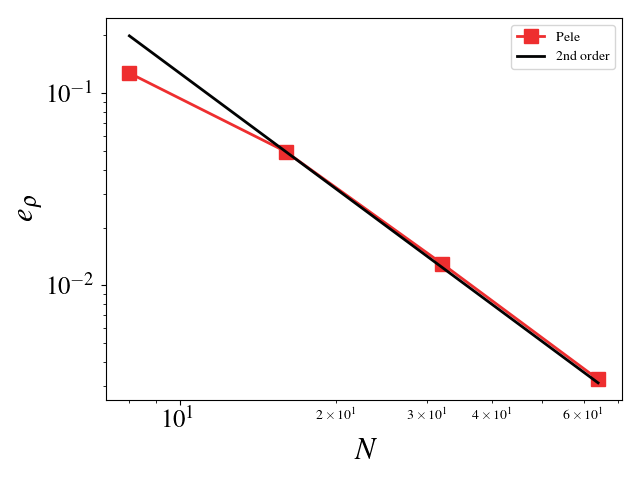
\includegraphics[width=\textwidth]{./rho_error.png}
    \caption{Density.}%
    \label{fig:}%
  \end{subfigure}%
  \begin{subfigure}[b]{0.49\textwidth}%
    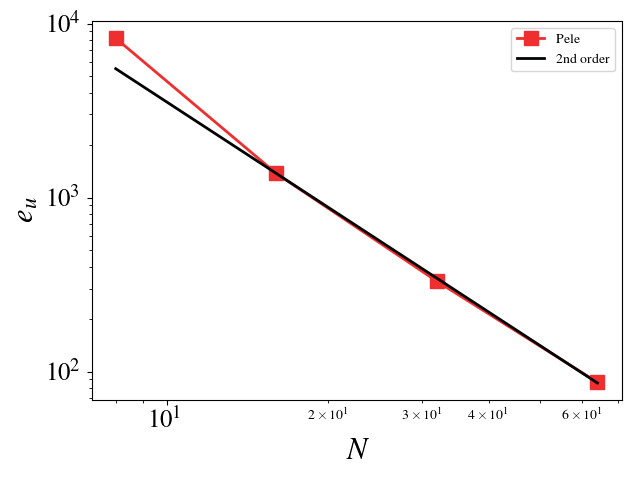
\includegraphics[width=\textwidth]{./u_error.png}%
    \caption{$u_1$.}%
    \label{fig:}%
  \end{subfigure}\hfill%
  \begin{subfigure}[b]{0.49\textwidth}%
    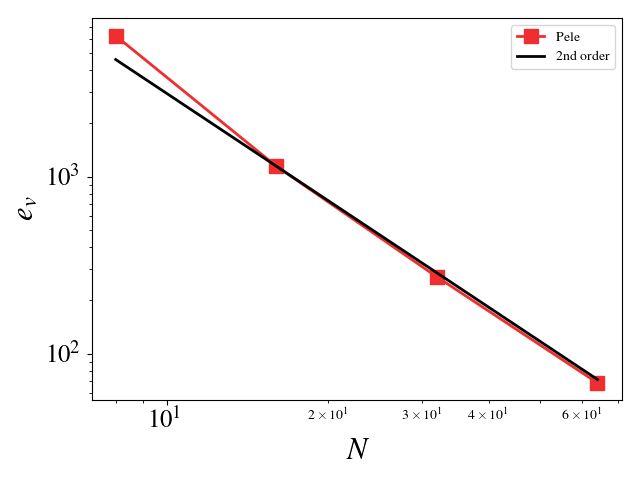
\includegraphics[width=\textwidth]{./v_error.png}%
    \caption{$u_2$.}%
    \label{fig:}%
  \end{subfigure}\hfill%
  \begin{subfigure}[b]{0.49\textwidth}%
    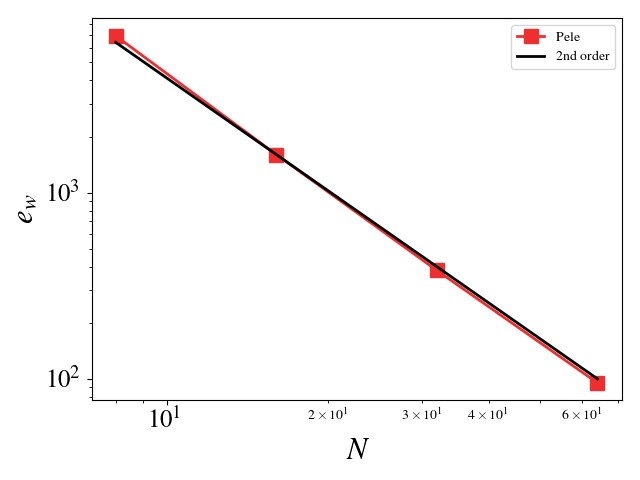
\includegraphics[width=\textwidth]{./w_error.png}%
    \caption{$u_3$.}%
    \label{fig:}%
  \end{subfigure}\hfill%
  \begin{subfigure}[b]{0.49\textwidth}%
    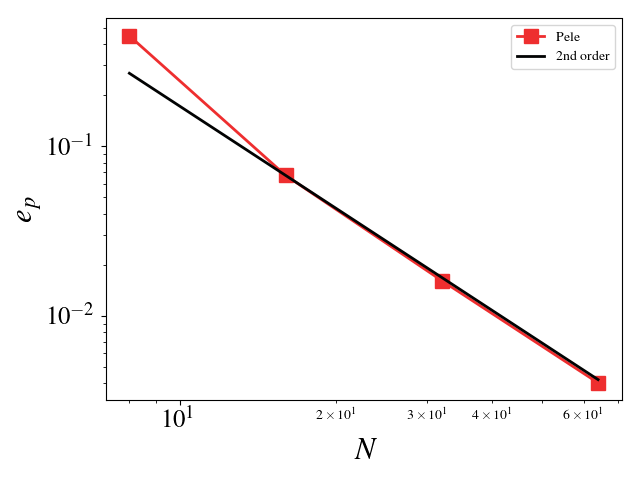
\includegraphics[width=\textwidth]{./p_error.png}%
    \caption{Pressure.}%
    \label{fig:}%
  \end{subfigure}\hfill%
  \caption{$L_2$ error as a function of $N$, the number of elements per side of the cube.}%
  \label{fig:results}%
\end{figure}%

\end{document}

